\chapter{Introduction}

Among all the tasks when designing a game, level design choices are some of the
most important \cite{blezinski2000, smith2008}. A well-designed level pushes a games' mechanics to its limits,
excites the player, and makes a good game great. A great example is the original
\emph{Super Mario Bros.} game. Only the first level sees the introduction of new
game mechanics, and afterwards new enemies are slowly introduced. However, the
number of units sold indicates that players found it to be a wortwhile and
rewarding game in sprite of the limited number of mechanics \cite{shaker2011}.

Level designers need to have knowledge across the spectrum of skills applicable
in game design \cite{blezinski2000}. They need an understanding of the game's mechanics, to know how
the artifical intelligence behaves, and to incorporate art assets into their 
levels in order to match the vision of the creative lead. Additionally, level
designers often have to switch between two considerations that constantly need
their attention: "Is this a good test of the skills that the player has
developed at this point in the game?" and "Does this obstacle fit with the
overall pacing and rhythm of the level?". Level designers frequentlly have to
use an iterative "modify and test" approach for certain game genres, as a small
change can sometimes have a large impact on the playability of a level \cite{smith2010}.

In spite of the importance of this task, the software for level designers has only
improved marginally over the years. In 2D games, the software is similar to many image
manipulation programs. For instance, in \emph{Super Mario Maker}'s level editor (which
can be seen in \autoref{fig:mm-editor}), the level designer drags terrain around with the resize and
translate handles, or uses drag and drop to place entities onto the map from a palette.
A similar comparison can be drawn for 3D level editors such as \emph{Trenchbroom}. In
Trenchbrrom, the level designer builds geometry as if they were creating a 3D model, then
moves around entities as they please. Level editing in both cases is a direct manipulation
task, but far too often level editors lack feedback that could help the designers more
quickly identify and correct mistakes, to the detriment of the efficiency and pleasure of
associated with level editing as a direct manipulation task \cite{schneiderman1983}. It is my
opinion that it would be more beneficial to the level designer if immediate feedback was 
provided on the level before playtesting begins, so problems could be eliminated as they
appear. One example would be to inform the level designer of levels that are not playable
before the designer runs playtesting. The need for better level editing tools is made
apparent by other software that has lowered the barrier for entry in the game development
industry such as the wide variety of open source game engines, intelligent development
environments, visual programming interfaces, and frameworks available to developers.

\begin{figure}[ht]
    \centering
    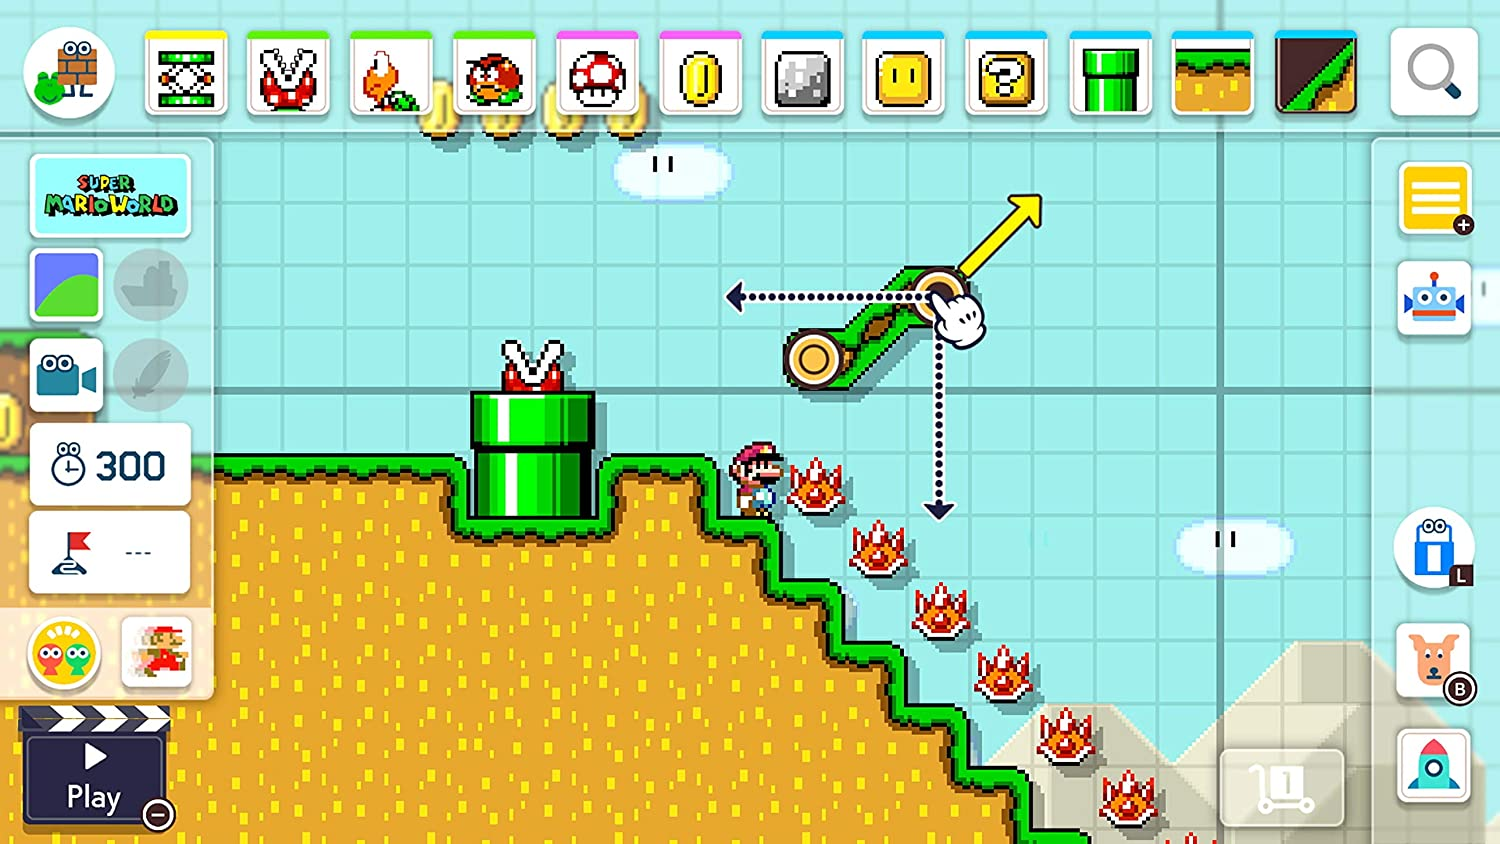
\includegraphics[width=0.8\textwidth]{img/fig1-mm-editor.jpg}
    \caption{\emph{Super Mario Maker}'s level editor.}
    \label{fig:mm-editor}
\end{figure}

One approach that is often implemented for level creation is procedural content generation.
Procedural content generation refers to the use of an algorithm to generate many kinds of
content \cite{shaker2016}. It has been used for terrain in 3D games like 
\emph{No Man's Sky}, dungeons in \emph{The Binding of Isaac}, complete worlds such as in
\emph{Endless Web} \cite{smith2013}, and even entire games like \emph{Yavalath}
\cite{browne2011}. Procedural content generaTion is a very versatile tool. One of the
motivations of the field is to create content much more quickly than ahuman can, and to
generate ideas that a human game designer may not have been able to come up with by
themselves. Procedural generation has been used in the past due to memory constraints - it
is more space efficient to store a single integer as a seed, and to generate a world at
runtime using it \cite{shaker2012}. \emph{Elite} used procedurally generated worlds to deal
with memory limitations. Roguelike games such as \emph{Hades}, and \emph{Risk of Rain 2}
commonly use procedural generation. The wide variety of encounters to explore due to the
stochastic nature of procedural content generation can be very engaging, and in the case of
games like \emph{Spelunky}, it can take hundreds of games to explore the entire procedural
space \cite{kazemi2009b}. In commercial platforming games, it is not very common to see
procedural generation used \cite{compton2006}, in spite of the increase in the amount of
content, replayability value, and development time saved by its use.

Shaker et al. describe a number of desirable properties of content generators \cite[6-7]{shaker2016}.
These properties include speed, controllability, reliability, expressivity and diversity,
and creativity. The importance of each property depends on the application. As an example,
a level generator that creates platform games at runtime needs to be fast. It needs to be
reliable so that there is a guaranteed route through a level. Additionally, it should be
creative, so that the levels it generates remain interesting over time.

Procedural content generation has been previously split into a taxonomy by Togelius et al.
\cite{togelius2011}, and this taxonomy is useful for describing content generators. The 
taxonomy is summarised in \autoref{table:pcg-taxonomy}. Level editing tools are one example
of offline content, and this category also includes games that ship with level editors.
Adapative content generation is present in \emph{Left 4 Dead}. The number and difficulty
of enemy encounters scale according to how well the players perform, so the content
generator adapts to different groups of players. Content generators that use evolutionary
algorithms or gramars make use of a generate and test approach, while chunk-based generation
approaches are normally constructive.

%\begin{table}[ht]
%\caption{Taxonomy of procedural content generation}
%\label{table:pcg-taxonomy}
%\begin{tabularx}{\textwidth}{| l | X | X |}

\begin{longtblr}[
    caption = {Taxonomy of procedural content generation},
    label = {table:pcg-taxonomy},
]{|c|X|X|}
\hline
\SetCell[c=1]{c}{Property of generator} & \SetCell[c=2]{c}{Possible values of property} \\\hline
Moment of content creation & Online - Content created during playtime & Offline - Content is either created separately, or during development. \\\hline
Type of content & Necessary - The produced content is required to play the game. & Optional - The game is playable without the generated content. \\\hline
Dimension of control & Random - The generator is not controllable by a user to any exten. & Parameterized - The user may set parameters which affect the generator's output. \\\hline
Applicability & Generic - The generator's output can be used in many contexts, or is applied to many different conditions. & Adapative - The content of the genetor adapts to different conditions. \\\hline
Reproducibility & Stochastic - Knowing the input conditions of the generator is not sufficient for prediciting the output. & Deterministic - Knowing the input conditions of the generator is sufficient to predict its output. \\\hline
Level of authorship & Mixed - The generator may require or optionally use input from a user. & Automatic - The generator is capable of producing content autonomously. \\\hline
Production approach & Generate and test - The generator constructs a large number of potential solutions and searches for an optimal selection. & Constructive - The generator sequentially constructs an acceptable solution. \\\hline
\end{longtblr}
%\end{table}

Platformer games are often the subject of papers on level generation for video games. A
platformer is a set of physics-based dexterity challenges that are viewed from the side
\cite{shaker2011}. The player navigates their avatar past obstacles, collects currency,
defeats enemies, and proceeds to the end of the level. Platformer games often have many 
short levels that the player must complete before finishing the game. These levels are
often time restricted, may or may not have checkpoints, and often implement a system where
the player can make a finite number of mistakes before having to restart from the beginning,
as is the case for both Super Mario Bros. and \emph{Crash Bandicoot}. In some game genres,
it is a challenge to evaluate the difficulty of a task at a glance, but a player familiar
with a platformer game can quickly gauge the challenge presented by a task, as the hazards
need to be visible in order for the player to react to them adequately \cite{sorenson2010}.
As an example, given a level in Super Mario Bros., a player knows that falling down a pit 
will instantly kill them, and can reason that larger pits make for a greater challenge.
Computers do not have the same level of intuition that experienced human players have about
the task, and it can be difficult to model a player's behaviour to generate appropriate
levels for them \cite{shaker2011}, which makes procedural content generation for platformers
such an interesting undertaking. Furthermore, the rules and actions present in platformers
are often simple (for instance, the primary actions in Super Mario Bros. are running and
jumping), but creative level geometry and enemy placement can lead to a large variety of
enjoyable content, despite the limited actions \cite{dahlskog2012}.


\subsection{Procedural generation for platformers in a selection of games}

There have been several interesting platformer games that have used procedural content 
generation. To start, two notably openly available platformers that incorporate content
generators are \emph{Infinite Mario Bros.} and Spelunky.

Infinite Mario Bros. has been frequently used in the past by the research community
\cite{shaker2011}. It is a public domain clone of the original Super Mario Bros. game. The
asserts are still proprietary, so this report will use \emph{InfiniteTux}, which is a version
of Infinite Mario Bros. using open-source assets. In InfiniteTux, levels are generated
automatically, and they slowly scale in difficulty by increasing the frequency of more
difficult terrain and adding more challenging enemies. Terrain generation proceeds in
several passes. First, the base of the level is generated from left to right by placing
human-authored platformer patterns in a random fashion. Each chunk has a small amount of
variety to it as well, but two chunks of the same category are generally very similar.
Some chunks are weighted higher than others depending on the difficulty parameter.

In \autoref{fig:ift-chunks}, the various chunks that InfiniteTux's generator uses are given.
From left to right, there are straight, hill straight, jump, tubes and cannones. Straight is
the most common chunk. Jumps, tubes, and cannons are considered by the generator to be more
difficult terrain, so these are added more often when it is desirable to increase the game's
difficulty.

\begin{figure}[ht]
    \centering
    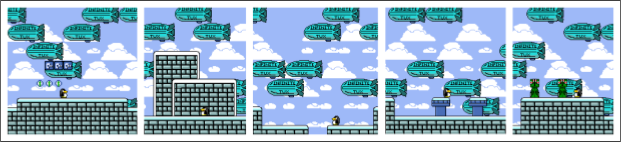
\includegraphics[width=\textwidth]{img/fig2-notch-chunks.png}
    \caption{Possible chunk types in \emph{InfiniteTux}}
    \label{fig:ift-chunks}
\end{figure}

A level is constructed by connecting enough chunks to fill the desired level width. The
chunks are chosen in a random fashion, with weights making some more common than others.
After placing these initial chunks, a second pass over the level is performed. For every
straight and hill straight chunk, a line of enemies can be added. It is also possible that
coins, a series of reward blocks are placed, as is the case in the leftmost image of 
\autoref{fig:ift-chunks}. The placed enemies depend on the difficulty of the level. More
difficult enemies hurt Mario when he jumps on them, avoid falling off ledges, or have wings,
providing them a jumping attack and an extra point of health. In \autoref{fig:ift-levels},
two levels generated with the same difficulty are shown. Notice that patterns repeat
frequently, like having a ceiling above several coins, the use of hills, and the flat
appearance of the two worlds. There appears to be a low amount of variety in the procedural
space of this generator. However, the generator is very reliable. Adjacent chunks are never
generated more than a few blocks above or below the previous, and celings cannot extend to
the last tile of a chunk, so each level is guaranteed to be winnable.

\begin{figure}[ht]
    \centering
    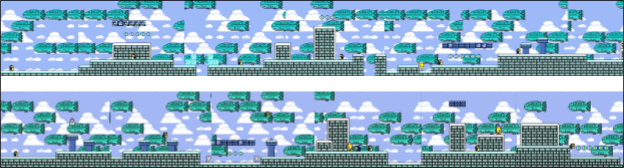
\includegraphics[width=\linewidth]{img/fig3-notch-levels.png}
    \caption{Two levels generated with similar parameters in \emph{InfiniteTux}}
    \label{fig:ift-levels}
\end{figure}

Spelunky is a very different game than InfiniteTux, but the two geenrators share many
similarities. The gameplay of Spelunky encourages exploration, and allows more ways for a
player to traverse the space, including destroying large amounts of terrain with bombs, and
using ropes to ascend high walls. As a result, it is easy to guarantee that a Spelunky
level is winnable. Spelunky always starts the player at the top of the screen, and the exit
is at the bottom, so rooms can be chosen in such a way that there is a guaranteed path
downward toward the exit. Levels in Spelunky are composed of 16 equally sized chunks
arranged in a 4x4 grid \cite[49-51]{shaker2016}. The chunks contain hooks that subsequent
passes of th generator use to place enemies, traps, or rewards. Due to playability
constraints, it is possible for a player to recall every level configuration in
approximately 500 playthroughs of the game \cite{kazemi2009a}. An example annotated
level is provided in \autoref{fig:spelunky}, which has each chunk numbered by its type, 
and a red line indicating a path to the end of level.

\begin{figure}[ht]
    \centering
    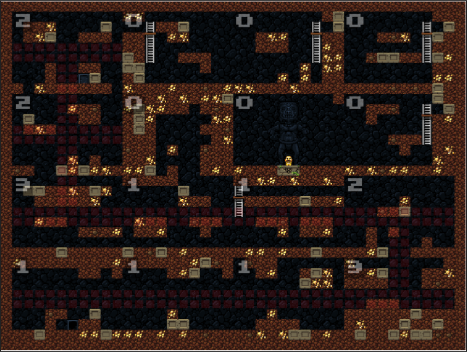
\includegraphics[width=0.8\linewidth]{img/fig4-spelunky.png}
    \caption{Level generated in \emph{Spelunky}. From \cite{kazemi2009a}}
    \label{fig:spelunky}
\end{figure}

\thesubsection{Procedural generation for platformers in research}
Compton and Mateas produced one of the first conceptual models for platformer game levels
\cite{compton2006}. In turn, their model is inspired by a model from music theory for
representing complex patterns in African and African American music. The model separates
platformer levels into atomic components, such as platforms, hills, and vines. In other
research, components are referred to as "beats" \cite{dahlskog2012, smith2008}. Beats are
grouped into patterns, chunks, or rhythm groups \cite{dahlskog2012}, which are sequences of
gameplay terminated by a break in rhythm. Rhythm groups can be combined into a unit called a
cell, which is one or more separate patterns placed together in a linear sequence. Cells can
be connected in a variety of ways, which produces a non-linear level. The researchers also
define a level design algorithm based around the rhythm model. The algorithm proceeds by
creating a context-free grammar to represent cells and rhythm groups. Each cell is connected
with some possible pattern like a branch, or a parallel pattern. Within each cell, zero or
more rhythm groups are placed, each with its own series of beats. A grammer that implements
this algortihm is later created by Shaker et al. \cite{shaker2012}. Later, Smith et al.
published work that extended the rhythm group model to be more complete \cite{smith2008}.
Their research clarifies the meaning of rhythm group to be more precise. A rhythm group ends
when there is a change in the rhythm of a level, such as if the player has reached a safe
zone from a previously unsafe zone. In \autoref{fig:hk}, a cell of \emph{Hollow Knight} is
shown with its rhythm groups represented by non-overlapping green regions.

\begin{figure}[ht]
    \centering
    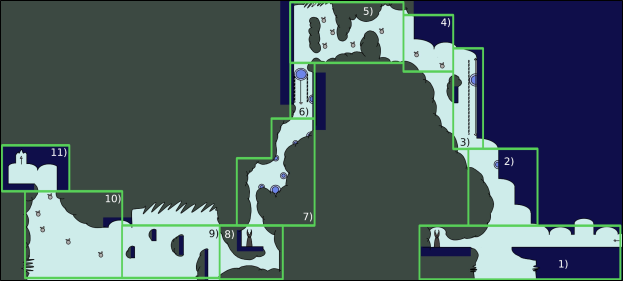
\includegraphics[width=\linewidth]{img/fig5-hk-rhythm.png}
    \caption{A single-cell level from \emph{Hollow Knight}}
    \label{fig:hk}
\end{figure}

The individual rhythm groups of the cell in \autoref{fig:hk} are described in detail:
\begin{enumerate}
    \item The player starts on the right hand side of the screen. The rhythm group extends out until the statue.
    \item The player must wall jump alongside the ceiling's right angles. The rhythm group ends after the saw blade, as they can stall here by nail-jumping on the saw for a break.
    \item The player reaches this rhythm group after wall jumping and dashing to it. They must avoid the moving saw blade along the wall. The rhythm group ends at the peak of the wall, as they can wall jump until ready for the next part.
    \item This rhythm group contains two flies that the player must bounce on to traverse it. It ends after the double jump off the second fly to reach the wall.
    \item This rhythm group extends from the wall in the top right, to the area above the moving saw blades. The player must use their dash and bounce off the flies, until reaching the left wall.
    \item Here, the player must slip past the moving saw without hitting the static saw. Then, they can rest by jumping against the wall.
    \item In this rhythm group, the player must bounce off the saw blades and slip through the narrow passage until reaching the statue.
    \item This rhythm group contains the status and the long dash wall.
    \item This rhythm group contains the 4 vertical walls. The player must climb each wall and dash to the next one.
    \item This rhythm group contains 5 flies that the player must bounce on, and dash between.
    \item The last rhythm group is the final platform containing the cell exit.
\end{enumerate}

Smith would later create a level generator based around the extended rhythm framework 
\cite{smith2011}. The \emph{Launchpad} generator outlined in the work uses two grammars, one
for generating beats, in the form of actions that the player performs. Beats have a start
time and a duration. The next part of the generation phase is geometry generation that
creates a level from the generated beats. Snice generation by grammars is fast compared to
other methods, a large number of levels are created, and two critics that evaluate the levels
find a optimal level that is playable and not flat. Important conclusions from this work
include the call for quantitative evaluations of analysing levels, instead of qualitative
measures, as well as the use of difficulty analysis in a generator.

An extension to Launchpad is \emph{Polymorph} \cite{jennings-teats2010}, which is a game
that uses Launcpad for dynamic difficulty adjustment. A limitation of Polymorph that is
cited by the authors is that difficulty is measured per beat, and does not consider how
adjacent beats might interact with each other to become more challenging. As an example,
jumping from a moving platform onto a platform containing a moving enemy is more complex
than landing on an empty platform, or avoiding the enemy without having to dismount the
platform.

Another interesting application of Smith et al. was \emph{Tanagra}, a "mixed-initiative
design tool...in which a human and computer work together to produce a level" 
\cite{smith2010}. Tanagra is pictured in \autoref{fig:tanagra}. Tanagra allows a human
designer to work with a procedural generator, while validating level playability, generating
alternative designs, and allowing re-generation of specific level segments. To describe it
in terms of the procedural generation framework \cite{togelius2011}, Tanagra is offline,
constructive, and uses mixed-authorship. A notable feature of Tanagra is the beat editor.
Where most level editors operate by placing individual tiles, Tanagra allows its users to
modify its generated beats as a whole. Level generation in Tanagra proceeds as follows:
1) Generate a level, 2) Respond to designer input by placing a moving existing geometry, 3)
Respond to the designer by modifying the beats of the level, 4) Ensure all levels are
playable. The authors call for additional extensions to Tanagra, including some form of
automatic difficulty analysis, the ability to view level paths, and support for more types
of rhythm groups.

\begin{figure}[h]
    \centering
    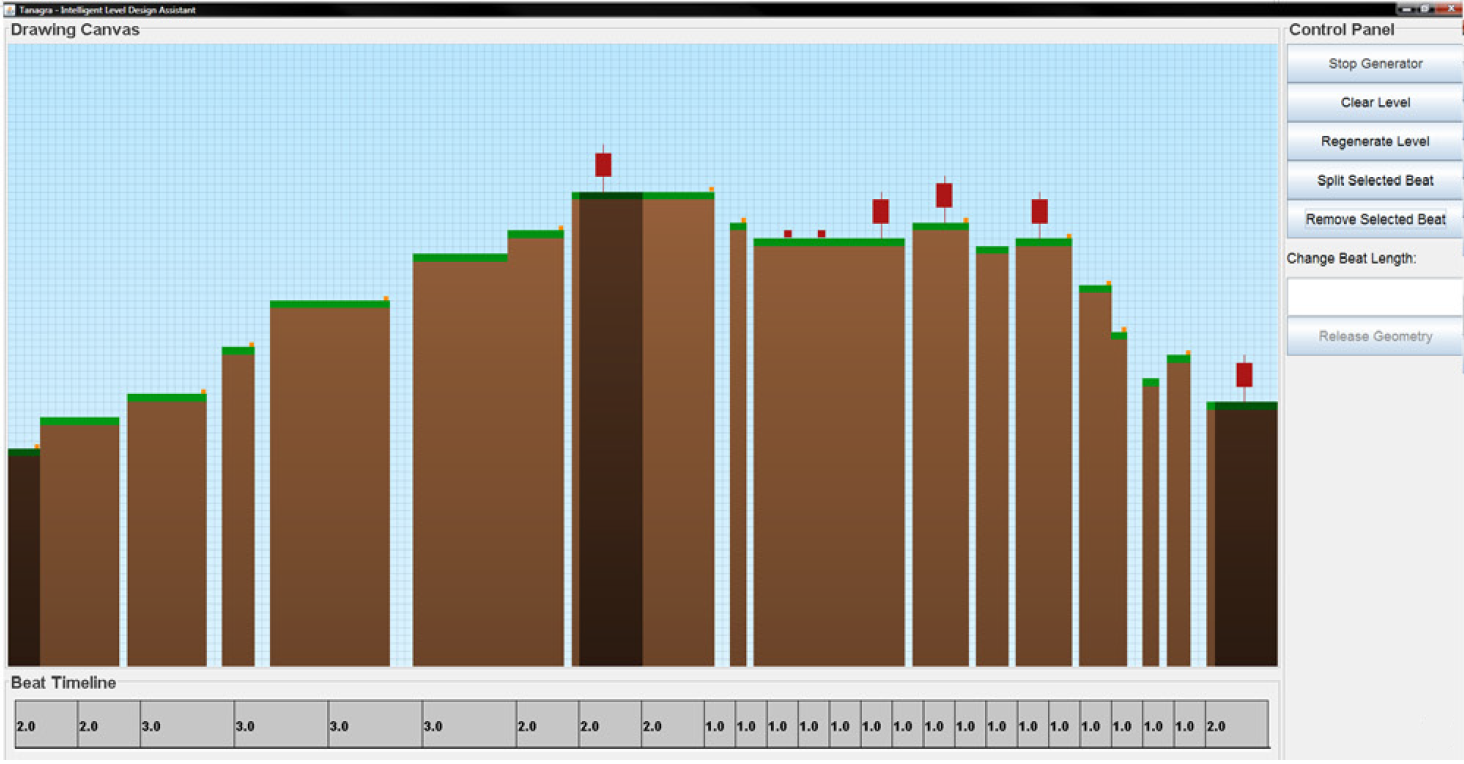
\includegraphics[width=\linewidth]{img/fig6-tanagra.png}
    \caption{Interface of \emph{Tanagra}. From \cite{smith2010}}
    \label{fig:tanagra}
\end{figure}

In 2010, the Mario AI Championship was held \cite{shaker2011}. The competition had several
tracks, including participants competing to create agents that could play procedurally
generated levels well, and participants competing to create level generators that produced
the most enjoyable experience, as determined by pairwise comparisons using 15 judges.
Six teams participated in the competion, each contributing to the report to document their
methodology.

The winner was Ben Weber, who created the "Probabilistic Multipass Generator". His approach
involved five passes from left to right over a level, which created the ground, hills, 
pipes, enemies, blocks, and then coins. each pass, some event is chosen from a uniform
distribution. A constraint exists that limits events so that the level remains playable.

Players were asked to play levels before testing the generators, and gameplay metrics were
available to competitors to incorporate into their algorithms. Shimizu and Hashiyama used
the player data to estimate a player's skill level, and to describe how likely they were to
break blocks, collect coins, and kill enemies. Sections of human-authored content were then
strung togther according to the player's playstyle. Shimizu and Hashiyama cited that the
benefits of this approach were a better fitting between a player's playstyle and skill, and
no complex fitness function. The authors state that the primary weakness is that the
expressivity of the levels is limited by the chunks available.

The next approach was by Sorenson and Pasquier, and is detailed in \cite{sorenson2010}.
Their method used an evolutionary algorithm to generate rhythm groups, which uses a fitness
function that estimates the difficulty of a rhythm group according to the margin of error
associated with jumps. At the same time, the fitness function is biased to select levels 
where the challenge alternates between successive rhythm groups. They assessed their model
on how successful it was at generating levels with a similar difficulty curve to the first
four levels Super Mario Bros., under the assumption that these first four levels are 
examples of well-designed Mario levels. Their generation took several hours, using an 
initial population of 200 individual levels evolving for 10,000 generations. For any
interactive software, this amount of delay is unacceptable, so the approach is more suited
for use in an offline generator.

Another intersting level generation approach was Peter Mawhorter's entry, which is expanded
upon in \cite{mawhorter2010}. The authors describe their approach as occupancy-regulated
extension (ORE). They use a variety of chunks, which are annotated with a frequency in which
they will be selected, and have additional metadata for the generator in the form of 
"anchors". Anchors represent possible places that the player might occupy in a chunk, and the
generator tries to preserve these places. Three main steps occur in the generation process.
Context selection chooses an existing anchor point in the level to expand starting with the
two intial anchors that mark the beginning and end of a level. Next, chunk selection occurs,
which determines which chunk from the library should be placed into the context. The last 
step is to integrate the chunk into the existing level. Post processing steps are also 
applied to generated levels to ensure that constraints are repsected, such as power-ups not
being too close together. The ORE generator occasionally produces some emergent or clever
level design. In \autoref{fig:clever-ore}, a strange powerup block was placed that only 
allows small Mario to reach or as normal Mario with a crouch-jump. The authors state that
the strength of their algorithm is game independence, since the generator only considers
anchor points, and the post-processing controls game-dependent constraints. They also state
that tagging the chunk libarry with keywords that provide some more information about each
chunk in the library may allow difficulty to be incorporated into generation. The authors
mention that ORE could easily be adapter into a collaborative or mixed-initiative system,
as the generation could interrupted as long as anchor points are preserved. Some of
weaknesses cited include the large chunk library needed for variety in the level; the
authors 42 chunks , which were all human-authored. Additionally, there is no strict
guarantee that the generated levels are playable.

\begin{figure}[h]
    \centering
    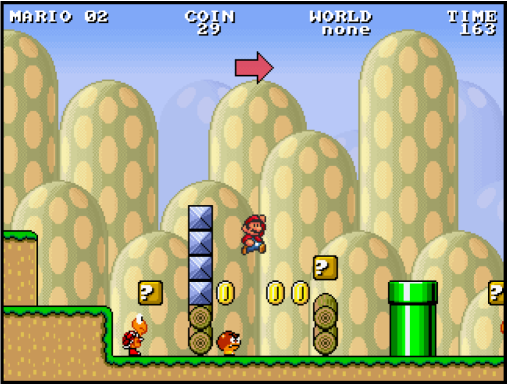
\includegraphics[width=\linewidth]{img/fig7-ore.png}
    \caption{Example of emergent behaviour in ORE's generated levels}
    \label{fig:clever-ore}
\end{figure}

\subsection{Computers in the creative process}

Computers have supported people creators for some time. Software that helps users in design
tasks is commonly referred to as computer-aided design software, or CAD. The motivating
ideas behind CAD are to provide users with a way of visualising their designs on the
computer, and to have the computer aid in applying constraints to the work
\cite{lawson1997}. Lawson and Loke argue that computers could do more to facilitate their
user's creativity in the design process, and provide three ways in which CAD systems could
contribute: "man/machine roles in creative thought", "parallel lines of thought", and "mind
sharing".

In order to play a greater role in creative thought for a task, CAD systems can provide the
user with suggestions or new ideas that could enhance the quality of the design. In the
context of a level editor, the user could receive suggestions for enemy placement or
recommend that a power-up be placed. An example of such a system is \emph{rlbrush} \cite{delarosa2021},
which is a level editor for \emph{Sokoban}, a tile-based game where the goal is to push
boxes into holes. Its interface provides the user with several suggestions that can
optionally be implemented, but not with any rationale about why its suggestions were given.
The system is shown in \autoref{fig:rlbrush}, and several different suggestions are visible
above the working canvas.

\begin{figure}[h]
    \centering
    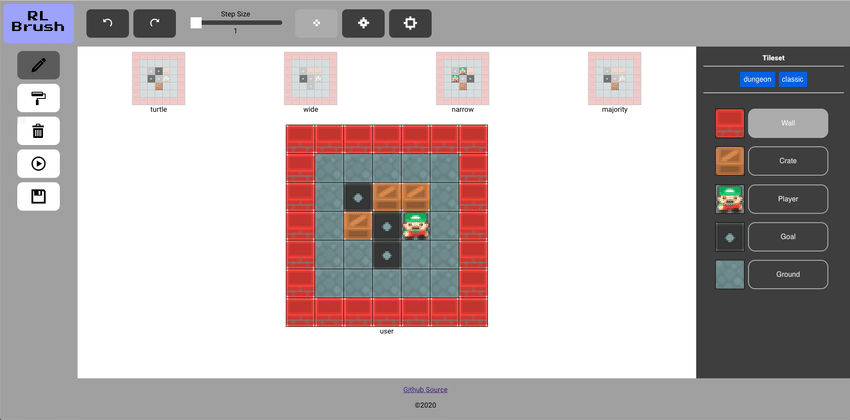
\includegraphics[width=\linewidth]{img/fig8-rlbrush.png}
    \caption{Interface of the \emph{rlbrush} editor for \emph{Sokoban}. From \cite{delarosa2021}}.
    \label{fig:rlbrush}.
\end{figure}

Parallel lines of thought refers to a system playing more than one role in the design 
process at a time. Several roles are outlined, including critic, collaborator, and informer.
Existing level editors have had the software operate as a collaborator before \cite{guzdial2019, liapis2013, smith2010}.
Of the software, \emph{Sentient Sketchbook} operates as both a critic and a collaborator. It
enforces playability and informs the user of the fairness of the current map, while also
generating many alternatives as iterations on the user's design. The idea of CAD software
playing different roles was also discussed by Lubart \cite{lubart2005}. In the work, four
different roles are outlined: nanny, where the system guides the user, colleague:, where the
system works with the user, pen-pal, where the system helps the user to communicate their
ideas to others, and coach, where the computer acts as an expert system that helps to teach
the user.

The last point is mind sharing, which refers to the notion that two minds working together
are greater than the sum of their parts. This relates to CAD systems that learn from their
mistakes and successes, and learn the habits of their user to create better suggestions.
The \emph{Morai Maker} system described in \cite{guzdial2019} used three different types of
agents that aimed to learn their user's designs, and used this information to automatically
add to the user's levels. According to the study, the participants saw that the system could
bring value to their levels, and it would take the form of a collaborator, nanny, or manager.
The collaborator and anny works were similar to what had been described in Lubart's work.
The manager role arose from participants feeling that the system was giving them instructions,
or evaluating their performance.

When the user and system co-operate on a task, the system can be described as a "mixed-
initiative system", as both the system and user work together towards a goal \cite[p191-200]{shaker2016}.
Some systems placed more emphasis on the human role, while others more on the computer role.
A procedural content generator for levels that accepts some parameters at the start of the
process technically has the user take some initiative, but the majority of the work is done
by the content generation algorithm. Similarly, in the field of CAD, tools like \emph{Blender}
allow a user to rapidly create 3D models, and the computer can automate some work, but the effort
is mostly on the user's end. Mixed-initiative systems can also be characterised by how they
handle three types of initiative: task initiative, speaker initiative, and outcome initiative.
Speaker initiative refers to the mechanism for determining when the user takes a turn on
the task, verssu when the system takes its turn. The spearker initiative of the ORE level
generator \cite{mawhorter2010} would be a form of turn taking. The level generator does its
work, then the user decides whether or not to re-generate any sections. Outcome initiative
refers to the process of deciding how the work of the problem solution should be divided.

\emph{Baba is Y'all} is an example of a mixed-initiative system where the user and system
interact in a more equal manner \cite{charity2020}. An image of the interface is provided in
\autoref{fig:biy}. The system is able to make suggestions based on the history of all levels
that have been created by every user. It provides suggestions for rules to implement into
the game that have't been thoroughly explored. It is also capable of helping players find
levels with similar mechanics to struggling players. Baba is Y'all demonstrates speaker
initiative by allowing the user to work on a level and providing suggestions. The
suggestions happen asynchronously while the user edits, so the user would have to end their
turn for the system to incorporate its suggestions. In regards to the outcome initiative of
Baba is Y'all, the user decides whether or not to incorporate the system's suggestions, so
therefore the outcome initiative is managed entirely by the user.

\begin{figure}[h]
    \centering
    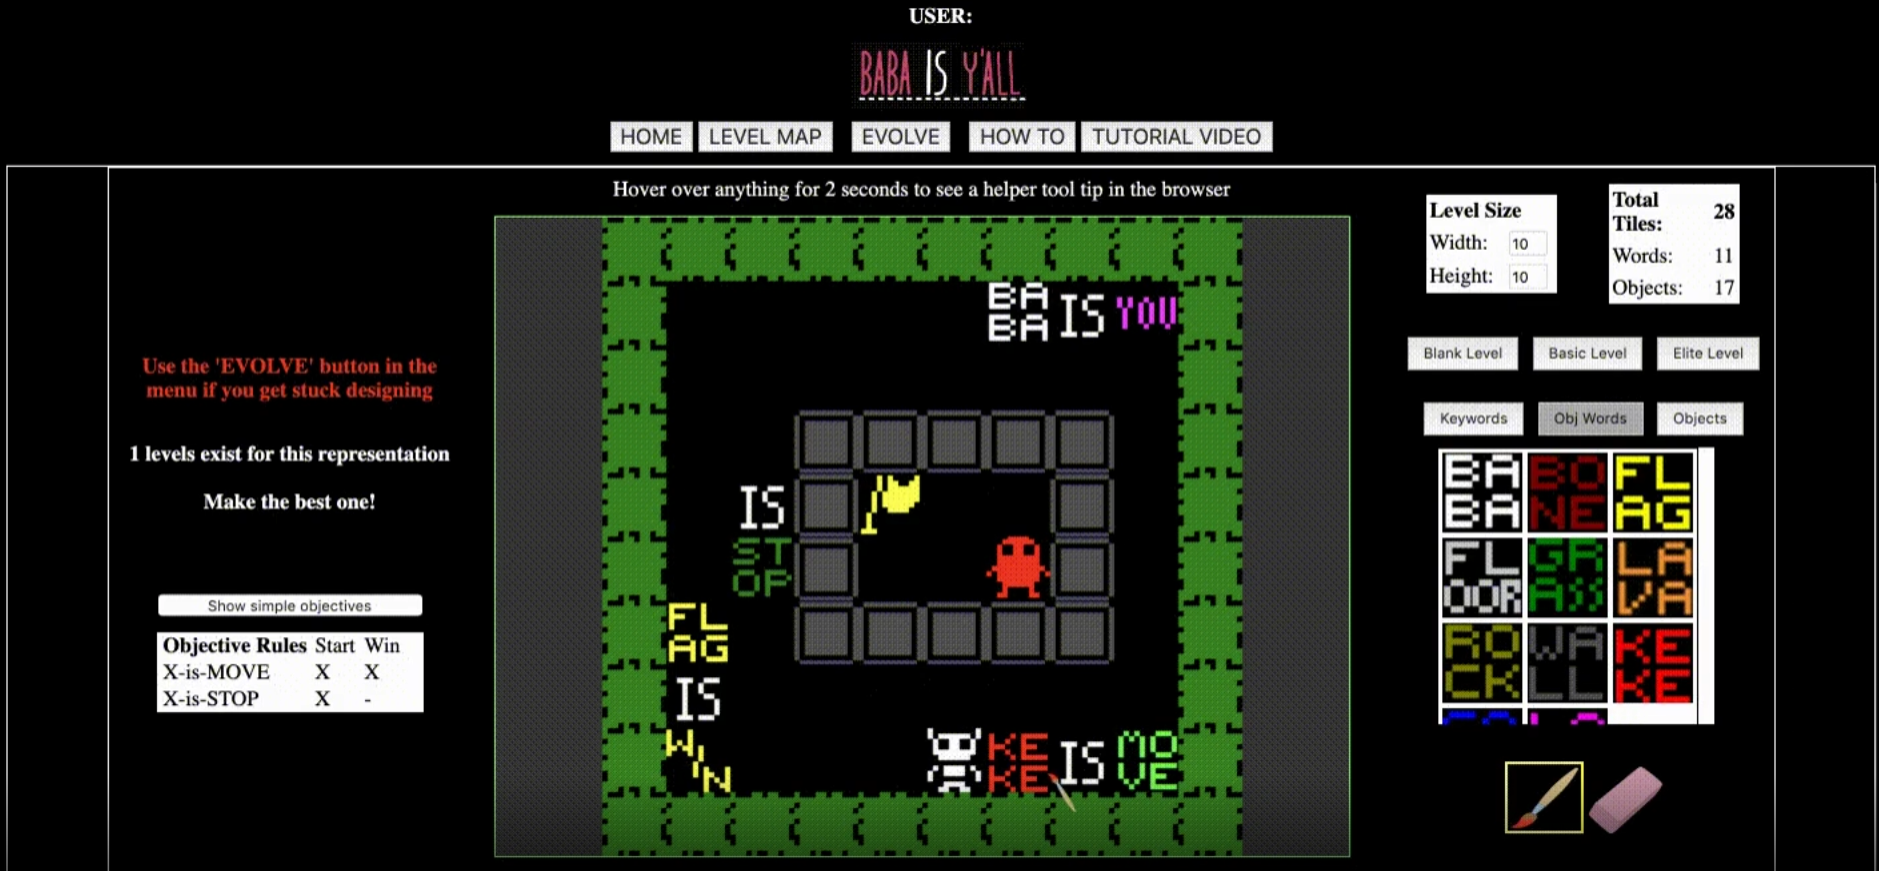
\includegraphics[width=\linewidth]{img/fig9-biy.png}
    \caption{Inteface of \emph{Baba is Y'all}}
    \label{fig:biy}
\end{figure}

\subsection{Functional and usability requirements}

For any interactive object or piece of software, it is important to consider the effect that
the interaction has on the user, and to design for a positive experience. A well-designed
interactive system is easy to understand, provides helpful feedback to its users about the
task, maps its controls in a sensible way, and clearly signifies how its controls can be used
to produce the desired effect \cite{norman2013}. Level editors as software fall under the
umbrella of interactive software, and as such are sensitive to these requirements.

A system's usefulness can be divided intor two areas, the utility it provides with its
functions, and its usability. Usability generally refers to the system's front end, while
utility refers to its back end. Many systems have utility, but less have usability. Nielsen
first proposed that a system's usability can be broken down into five areas which include
learnability, memorability, efficiency, satisfaction, and how successful the system is at
dealing with errors \cite[p22]{nielsen1994}. Learnability refers to the challenge associated
with the first time a user interacts with a system. Memorability refers to how easy it is
to remember how to use a system. An efficient system allows the user to perform their work
quickly, and is careful not to waste the user's time. A satisfying system feels pleasant to
usem perhaps by having a pleasant visual design, or by the user feeling that the system
helped them with their task. A system that effectively manages its errors provides helpful
error messages when appropriate, and tries to limit the amount of errors that can be made by 
the user.

A system's usability can be evaluated by how well it matches the ten usability heuristics
proposed by Nielsen in \cite{nielsen2005}. The heuristics attempt to measure the usability
principles outlined above, and include:

\begin{description}
    \item [Visibility of system status] The system should keep the user informed about its state, and provide feedback within a reasonable amount of time.
    \item [Match between system and real world] The system should use concepts and terminology that thte user would know. Information should appear in a natural and logical manner.
    \item [User control and freedom] Users often make mistakes, so the system should always allow the user to cancel actions, undo or redo, and be able to navigate backward.
    \item [Consistency and standards] The system should use standard language for common actions, and the same words should be used for the same actions.
    \item [Error prevention] A usable system constrains the number of errors a user can make.
    \item [Recognition rather than recall] The system should make relevant information visible to reduce the user's memory load. When possible, instructions should be available.
    \item [Flexibility and efficiency] Shortcuts should be provided in order for advanced users to save time.
    \item [Aesthetic and minimalist design] The system should only include features that add to the usability. Information that is not needed for the task should not be shown, as it can distract from relevant information.
    \item [Error recognition and recovery] Error messages should be clear and precise, and suggest a way to recover from or fix the error.
    \item [Help and documentation] Extra help should be easy to access, clear, and helpful.
\end{description}

These usability heuristics provide a set of best practices to follow when designing a user
interface. Usability is important in designing a level editor, because one of the main
goals is to aid designers in the process of levle design. A system with a lot of utility that
results in desirable outcomes may be discarded by users if they have a poor experience 
interacting with it \cite[p10]{norman2013}.

The method of interaction differs among software. In most level editors, designers interact
with a representation of the level, and iterate on their design by adding elements one at a
time. Often, these elements are accessed from a palette, as in popular level editors like
\emph{Halo Reach}'s forge mode, or Super Mario Maker. The designer often sees the components
as they appear in game, and can manipulate their position and properties through the interface
by using various tools. This type of interaction is called direct manipulation. Direct
manipulation was first by Schneiderman in \cite{schneiderman1983}. Schneiderman observed
office works using single line editors versus using display eeditors, where many lines could
be seen at once, and feedback on changes was immediate. Direct manipulation tasks involve
several characteristics. A continuous representation of the final object needs to be
available. Actions should be performed via button presses or mouse movement instead of by
text commands. Operations should be rapid, incremental, and reversible. The combination
of these properties leads to a high desirable outcome: experts can rapidly complete tasks,
users feel in control over the system, and users receive immediate feedback on the effect of
their actions, leading to the ability to experiment with their approach. Additionally, users
feel comfortable experimenting with the system because the cost of making a mistake is very
low. Most level editors meet the criteria for qualifying as a direct manipulation task, but it
can be hard to convey information about the experience that the level creates for the user
unless the designer plays it, so the cost of making a mistake is higher in terms of time lost,
which may lead to less experimentation on the part of the designer due to time constraints.

In a chapter about designing tools for game design, Rouse states,
\begin{quote}
In order to create superior content, the design team will need to be equipped with 
well-designed, robust game creation tools. Therefore, one can conclude that designing a
good game is about designing good game creation tools \cite[p392]{rouse2004}.
\end{quote}

In the rest of the chapter, Rouse outlines a number of requirements for any level-editing tool.
The first requirement is similar to Nielsen's usability principle of visibility. The designer
should be able to see the world being created while in the process of creating it. Level
editors should also provide the designer with extra information about the level, not
normally visible in game. The level editor in Halo: Reach allows the designer to see spawning
information about the objects they have placed. The Tanagra content generator provides
information about the pacing of the level to the user in the form of a beat timeline, which
visually represents the rhythm of the level \cite{smith2010}. A more dense beat timeline 
indicates a faster-paced level, since each beat is a player action like waiting or jumping.
Another helpful addition to level editors is the ability to immediately playtest the 
in-progress level. It is well-known that testing is a critical part of any software 
development, and this is particularly true for games, as gameplay is usually considered
the most important feature of a game. A final requirement is that a level editor should allow
the designer full control over all gameplay critical sections of a level. Without full control
over these sections, the level designer may become frustrated by seemingly arbitrary 
limitations getting in the way of their work.

THe goal of this project is to investigate how to design a system that can assist level
designers in creating better levels. As the general task of "creating better levels in video
games" is quite broad, the scope of this project will be imited to the platform game genre.
A significant amount of research has been spent analysing and developing level generators for
platformers, and given the 12-week period available for the project, it makes the most
sense to stick to the platformer genre. First, procedural generation methods will be examined
in-depth. Then, the use of computers in the creative process will be covered. It is also
important to cover the requirements of interactive systems in general, and then narrow in on
these requirements with respect to level editors. From these requirements, and the research
in the previous sections, a system will be proposed and implemented. The system will be a
level editor for InfiniteTux that aids the level designer in the design process, with the goal
of using procedural content generation. 

InfiniteTux was chosen for several reasons. As previously stated, InfiniteTux shares its
mechanics with Super Mario Bros., which has seen extensive attention in research due to
its popularity and events such as The Mario AI Championship. Another reason to improve
InfiniteTux is that the code is openly available under the GPL license. InfiniteTux is
implemented in Java, which is a language that is familiar to many programmers. Lastly, 
InfiniteTux already features an unfinished level editor, and an interface for generating
levels for the game. Specific functional requirements will be outlined later. After the
implementation of the system, it will be evaluated by how well it meets these functional 
requirements, as well as the amount of variation present between its generated levels.